\section{Recovering results}

\begin{figure}
    \centering
    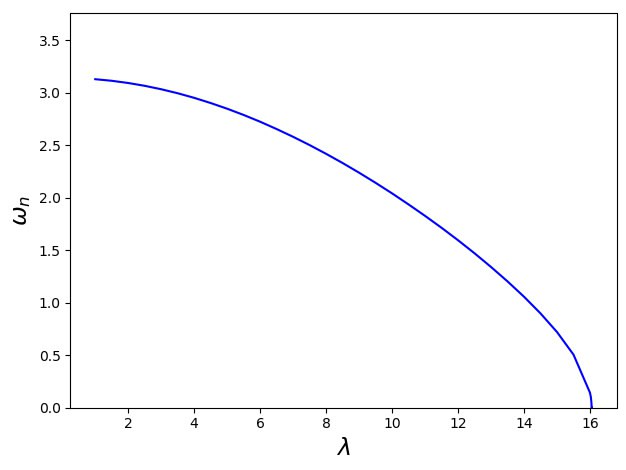
\includegraphics[width=0.5\linewidth]{figures/eigenvalues-external-field-approximation.png}     
    \caption{The energy of the modes as $\lambda$ increases, when ignoring the backreaction of the Klein-Gordon field to the background electric field. Using the stated method, we recover the results from \cite{Ambjorn1983}}.
    \label{fig:external-field-approximation}
\end{figure}

\begin{figure}
    \centering
    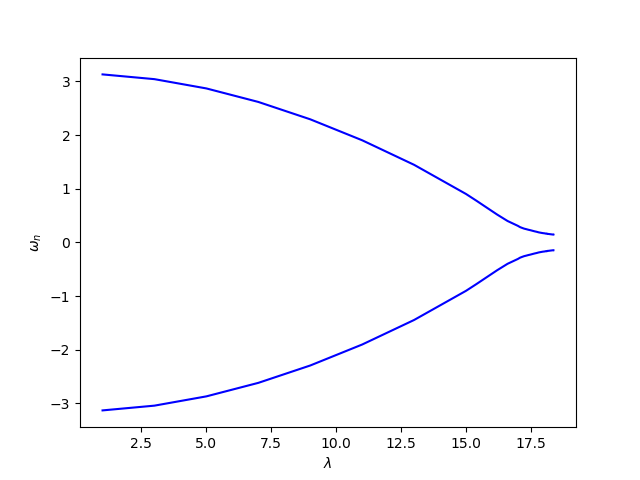
\includegraphics[width=0.5\linewidth]{figures/eigenvaluesAmbjorn.png}   
    \caption{The energy of the modes as $\lambda$ increases when taking backreaction into account, but only using one mode in the calculation of the vacuum polarization, and ignoring the extra $\frac{e^2}{\pi} A_0(z)$, as was done in \cite{Ambj1983}. }
    \label{fig:eigenvaluesAmbjorn}
\end{figure}

As a sanity check, we show in Figure \ref{fig:external-field-approximation} the behavior of the energy of the different modes of the Klein-Gordon field as the background electric field strenght $\lambda$ is increased. We also show in Figure \ref{fig:eigenvaluesAmbjorn} the recovered results from \cite{Ambj1983} that were calculated using the method discussed throughout Chapter \ref{cha:Vacuum-Polarization}.
